
%latest commented and above added for camera-ready
%\begin{figure}[t]
%\centering
%\includegraphics[scale=0.8]{synthetic-cdf-plots/dom0-forward-unseen-cdf.robust.eps}
%\caption{Prediction error CDF for \textit{colocated} Dom0 CPU estimation.}
%\label{fig:forward-unseen-cdf}
%\vspace{-0.25in}
%\end{figure}


In the previous section, we described the motivation and methodology
of developing models to predict colocated and 
dispersed CPU utilization.
After the models are built, we recompute or ``predict'' the colocated
CPU value for the training set itself, using the generated model 
coefficients. This is a sanity check to validate model correctness.
The results showed that well-fitting models 
were built, with less than 1\% to 2\% error for all workloads. However, the real test
is whether the models are able to successfully
predict the average CPU usage well, when applied to unseen data.
We present model evaluation on both synthetic data-sets and benchmark
application data in this section.


% 
% \begin{figure*}[t]
% \centering
% \noindent\makebox[\textwidth]{% 
% \begin{tabular} {cc}
% \includegraphics[scale=0.85]{synthetic-cdf-plots/domu-forward-unseen-cdf.robust.eps} & 
% \includegraphics[scale=0.85]{synthetic-cdf-plots/dom0-forward-unseen-cdf.robust.eps} \\
% (a) DomU forward model & (b) Dom0 forward model 
% \end{tabular}
% }
% \caption{Prediction error CDF for \textit{colocated} CPU usage estimation.}
% \label{fig:reverse-unseen-cdf}
% \end{figure*}
% 
% 
% \begin{figure*}[t]
% \centering
% \noindent\makebox[\textwidth]{% 
% \begin{tabular} {cc}
% 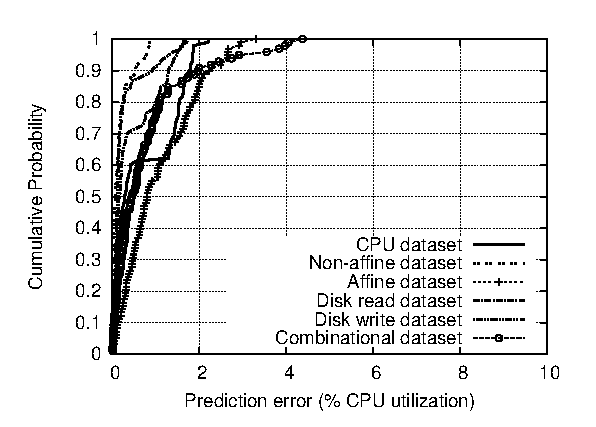
\includegraphics[scale=0.85]{synthetic-cdf-plots/domu-reverse-unseen-cdf.robust.eps} & 
% 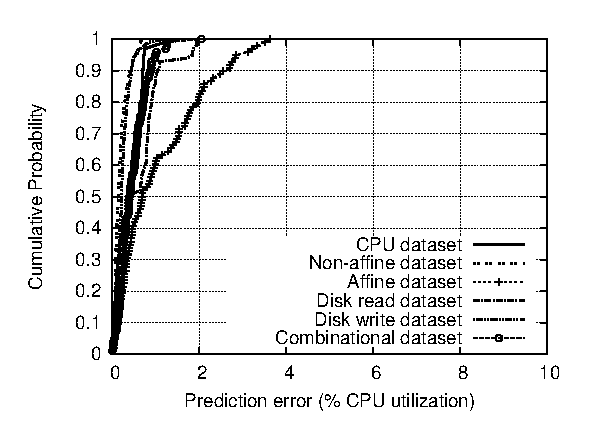
\includegraphics[scale=0.85]{synthetic-cdf-plots/dom0-reverse-unseen-cdf.robust.eps} \\
% (a) DomU reverse model & (b) Dom0 reverse model
% \end{tabular}
% }
% \caption{Prediction error CDF for \textit{dispersed} CPU usage estimation.}
% \label{fig:reverse-unseen-cdf}
% \end{figure*}

% \begin{figure*}[t]
% \centering
% \noindent\makebox[\textwidth]{% 
% \begin{tabular} {ccc}
% \includegraphics[scale=0.7]{aff-apps/rubis-co-domu1.eps} & 
% \includegraphics[scale=0.7]{aff-apps/rubis-co-domu2.eps} &
% \includegraphics[scale=0.7]{aff-apps/rubis-co-dom0.eps} \\
% (a) Web tier VM & (b) DB tier VM &  (c) Colocated Dom0 \\
% \end{tabular}
% }
% \caption{Estimating colocated CPU utilization for RUBiS using \textit{forward} models.}
% \label{fig:rubis-forward}
% \end{figure*}



% \begin{figure*}[t]
% \centering
% \noindent\makebox[\textwidth]{% 
% \begin{tabular} {rccl}
% \includegraphics[scale=0.65]{aff-apps/rubis-dis-domu1.eps} &
% \includegraphics[scale=0.65]{aff-apps/rubis-dis-domu2.eps} &
% \includegraphics[scale=0.65]{aff-apps/rubis-dis-dom01.eps} &
% \includegraphics[scale=0.65]{aff-apps/rubis-dis-dom02.eps} \\
% (a) Web tier VM & (b) DB tier VM &
% (c) Dom0 of Web tier VM & (d) Dom0 of DB tier VM \\ 
% \end{tabular}
% }
% \caption{Estimating dispersed CPU utilization for RUBiS using \textit{reverse} models.}
% \label{fig:rubis-reverse}
% \end{figure*}


% \begin{figure*}[t]
% \centering
% \noindent\makebox[\textwidth]{% 
% \begin{tabular} {cc}
% \includegraphics[scale=0.65]{aff-apps/rubis-dis-domu1.eps} &
% \includegraphics[scale=0.65]{aff-apps/rubis-dis-domu2.eps} \\
% (a) Web tier VM & (b) DB tier VM \\ 
% \includegraphics[scale=0.65]{aff-apps/rubis-dis-dom01.eps} &
% \includegraphics[scale=0.65]{aff-apps/rubis-dis-dom02.eps} \\
% (c) Dom0 of Web tier VM & (d) Dom0 of DB tier VM \\ 
% \end{tabular}
% }
% \caption{Estimating dispersed CPU utilization for RUBiS using \textit{reverse} models.}
% \label{fig:rubis-reverse}
% \end{figure*}



\subsection{Model evaluation with synthetic data-sets}
In this sub-section, we present our findings when the generated
models were applied to ``unseen'' datasets. 
By unseen, we mean that these datasets are not a part of the
input set for model creation.
The setup used for evaluation with synthetic\index{Synthetic benchmarks} 
data-sets is the same 
as the one that was presented in Section \ref{sec:arescue-setup}, 
for the benchmarking experiments.
We present the evaluation of the two approaches separately\textemdash{}predicting
total CPU usage, and predicting differential CPU usage.

\begin{figure}[t]
% \centering
\hspace{-0.2in}
\subfloat[Dom0 CPU in colocated scenario (colocation model)]{\includegraphics[scale=0.9]{arescue-figures/synthetic-cdf-plots/dom0-forward-unseen-cdf-robust.eps}}
\subfloat[Dom0 CPU in dispersed scenario (dispersion model)]{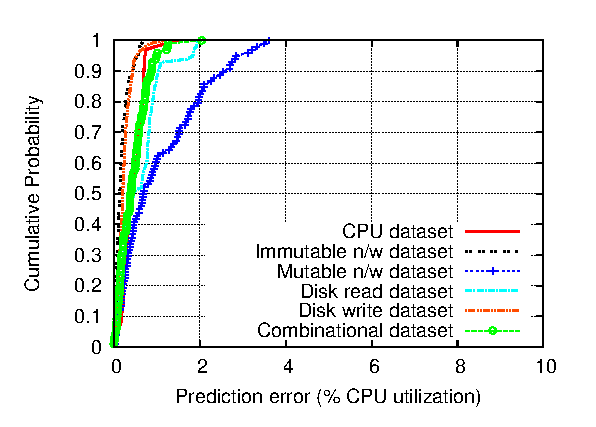
\includegraphics[scale=0.9]{arescue-figures/synthetic-cdf-plots/dom0-reverse-unseen-cdf-robust.eps}}
\caption{Prediction error CDF for Dom0 CPU estimation.}
\label{fig:dom0-unseen-cdf}
% \vspace{-0.25in}
\end{figure}

% We test the models on the following workload types \textemdash{} CPU,
% intra-PM traffic, inter-PM traffic, disk read, disk
% write and also on combinational workloads.
\underline{For models predicting total CPU usage:}
The training data input for the models was generated
by generating resource utilization at pre-defined discrete 
levels, however, the derived models
need to be applied to ``unseen'' resource usage profiles
in order to judge their adequacy. For this reason, the
CPU workload for testing consists of $100$ randomly
picked values in the range $1\%$
to $100\%$, the mutable\index{Mutable} and immutable\index{Immutable} 
Rx/Tx test workloads
are chosen randomly from the range 10 Mbps to 90 Mbps, the
disk read/write rates are randomly chosen from the range
0 to 1500 blocks/second, and the combinational workloads 
had randomly chosen values for each parameter (CPU, mutable
network traffic, immutable network traffic,
and disk) from these same ranges.

Fig. \ref{fig:dom0-unseen-cdf} plots the CDFs of error when
Dom0 \emph{colocation} and \emph{dispersion} models were applied to all the
six unseen datasets\textemdash{}cpu, mutable \& immutable network traffic, disk read,
disk write and combinational loads. It can be observed that
all the CDFs seem to stick to the left end of the graph, however,
the 90th percentile
error is around 3\% absolute CPU and maximum error is around 4\%. 
We plotted similar error
CDFs for colocated and dispersed DomU CPU estimation. In 
all cases, we found that
the 90th percentile absolute error was within 3\%. We do
not present all the CDFs here, for sake of brevity; they can
be found in the technical report at \cite{affine-modeling-tech-report}.
In case of Dom0 models\index{Dom0 model}, 
since the savings due to co-location
is significant (as concluded from the benchmarking results), an
accuracy with 3\%error might suffice for a good prediction. However, in
case of DomU models\index{DomU model}, 
the savings themselves being marginally 
lower (between 0 to 10\%), a 3\% error could imply higher 
relative error in comparison. 
% With further increase in affine 
% network rate, increased CPU utilization (and hence increased 
% savings) may still benefit from this model's accuracy.
% \begin{figure*}[t]
% \centering
% \noindent\makebox[\textwidth]{% 
% \begin{tabular} {ccc}
% \includegraphics[scale=0.65]{figures/unseen-cpu-cdf.eps} & 
% \includegraphics[scale=0.65]{figures/unseen-aff-cdf.eps} &
% \includegraphics[scale=0.65]{figures/unseen-nonaff-cdf.eps} \\
% (a) CPU dataset & (b) Affine dataset &  (c) Non-affine dataset \\
% \end{tabular}
% }
% \caption{Prediction error CDF for different datasets.}
% \label{fig:forward-unseen-cdf}
% \end{figure*}

\begin{figure}[t]
	\hspace{-0.6in}
	\centering
	\subfloat[DomU-1]{\includegraphics[scale=0.95]{jss-figures/aff-synth/synth-co-domu1.eps}}
	\subfloat[DomU-2]{\includegraphics[scale=0.95]{jss-figures/aff-synth/synth-co-domu2.eps}} \\
	\subfloat[Colocated Dom0]{\includegraphics[scale=0.95]{jss-figures/aff-synth/synth-co-dom0.eps}}
\caption{Estimating colocated CPU utilization for synthetic data-set}% on Xen.}
\label{xensynth}
\end{figure}


\begin{figure}[t]
	\hspace{-0.6in}
	\centering
	\subfloat[Web tier VM]{\includegraphics[scale=0.95]{jss-figures/aff-apps/rubis-3way-co-domu1.eps}}
	\subfloat[DB tier VM]{\includegraphics[scale=0.95]{jss-figures/aff-apps/rubis-3way-co-domu2.eps}}
	\\
	\subfloat[Colocated Dom0]{\includegraphics[scale=0.95]{jss-figures/aff-apps/rubis-3way-co-dom0.eps}}
\caption{Estimating colocated CPU utilization for RUBiS} % using \textit{forward} models.}
\label{fig:2ndchap-rubis-forward}
\end{figure}

\underline{For models predicting differential CPU usage:}
In order to generate
synthetic workload which closely emulates a real application
scenario, we spawn multiple client processes, each sleeping
for fixed intervals of time (emulating average think-time)
and generating request for transmission of varying number
of bytes or segment sizes. Thus, the artificial constraint
of each client process requesting only a single segment size
has been discarded. We generate randomly different load levels
using different number of client threads every minute, each
generating requests for different segment sizes
and monitor resource usage utilization
over a period of 18 minutes. As expected,
the resultant network traffic rates and
CPU utilization also vary.

Fig.~\ref{xensynth} shows colocated\index{Colocated}
CPU usage, predicted versus actual, for both DomUs and Dom0.
We can see that as dispersed CPU utilization
changes due to change in network usage, predicted colocated
utilization also varies similarly.
% Fig.~\ref{xensynth-cdf} shows
% the prediction error CDFs for DomU and Dom0 forward and reverse models
% when applied to this synthetic data-set. 
The maximum error in DomU prediction is within 1\% absolute
CPU usage for both DomUs (VM1 and VM2) and the maximum
error in colocated Dom0 prediction is within 2.4\% absolute CPU.
Since difference in CPU utilization for DomU is
quite low and therefore less interesting, we focus on Dom0
models here onwards.


\subsection{Model evaluation with application benchmarks}
The above evaluation with synthetic workloads demonstrated
that predicting the differential CPU usage, which considers
only the mutable network usage metrics (including both network rate
and segment size metrics) give higher accuracy predictions.
Hence, we use that approach for the rest of the evaluation
in this chapter.


%\begin{figure}[t]
%\centering
%\subfloat[Web tier VM]{\includegraphics[scale=1]{../ieeecloud2011/savefigures/aff-apps/rubis-co-domu1.eps}} 
%\subfloat[DB tier VM]{\includegraphics[scale=1]{../ieeecloud2011/savefigures/aff-apps/rubis-co-domu2.eps}}  \\
%\subfloat[Colocated Dom0]{\includegraphics[scale=1]{../ieeecloud2011/savefigures/aff-apps/rubis-co-dom0.eps}}
%\caption{Estimating colocated CPU utilization for RUBiS using \textit{colocation} models.}
%\label{fig:rubis-forward}
%% \vspace{-0.25in}
%\end{figure}


For evaluating our prediction models with an application benchmark, we 
chose RUBiS~\cite{rubis}\index{RUBiS}.
RUBiS emulates an auction 
website like eBay, and allows simulation of various users/clients who engage
in different tasks like user registration, item registration, browsing items,
bidding for \& buying items and so on. 
RUBiS is a two-tier application, consisting of a web tier and a database tier
that communicate with each other for servicing each user request. Each tier
is hosted in a separate VM. 
We generate repeatable RUBiS workloads in both dispersed and colocated cases,
and compare average resource utilization levels (predicted versus measured)
over 30-second intervals. The RUBiS workload consisted of 800 clients
generating site browsing load simultaneously, and requests being fired
at determined times.
As done in~\cite{profiling-and-modeling}, we also consider open-loop
applications, where the inter-arrival times of the sequence of requests 
is the same across the dispersed and colocated scenarios. 
This is the case when response times are far lesser than the minimum
think-time. The think-times are randomly chosen from a negative 
exponential distribution with a mean of 7 seconds, and minimum think-time
of 5 seconds.

Fig.~\ref{fig:2ndchap-rubis-forward} plots predicted and measured CPU
utilization for the web tier VM (Fig. \ref{fig:2ndchap-rubis-forward}(a)),
the DB tier VM (Fig.~\ref{fig:2ndchap-rubis-forward}(b)) and the
Dom0 CPU utilization (Fig.~\ref{fig:2ndchap-rubis-forward}(c)) after colocation.
As seen in the figure, the RUBiS workload consists of 3 phases. It starts
with an
up-ramp phase which lasts till the 10th interval and then starts climbing
to steady state. Prediction is able to follow the climb well. The
steady state lasts till the 27th interval and then begins the ramp-down
phase. Prediction follows the drop also pretty accurately.
The maximum error in CPU
usage prediction is less than $2\%$ for both Dom0 and DomU models.
% When the VMs were moved from colocated to dispersed, the 90th percentile error
% in prediction was $3\%$ and $4\%$ for Dom0 and DomU models respectively.
Similar graphs were plotted for \emph{dispersion} model as well and
maximum error is within 2\% absolute CPU utilization.
Thus, prediction accuracies for both Dom0 and DomU models are equally high.
indicating that the models
can be successfully applied to an application without training on that
specific application's resource utilization profiles themselves.

\begin{table}[t]
	\centering
	\caption{Model accuracy with varying load}
	% \noindent\makebox[\textwidth]{%
	\begin{tabular}{|c|c|c|c|c|} \hline
		\textbf{No. of} & \textbf{Maximum}  & \multicolumn{3}{|c|}{\textbf{Max error (\% CPU)}} \\  \cline{3-5}
	\textbf{clients} & \textbf{net-affinity} & \textbf{DomU} &  \textbf{Dom0} & \textbf{Dom0} \\
		 & \textbf{(Mbps)} &  &  \textbf{colo} & \textbf{disp} \\ \hline  %\cline{2-9}
  500 & 6.8 & 1.73 & 1.33 & 0.90 \\
	1000 & 13.4 & 1.50 & 0.98 & 0.82 \\
	1500 & 19.8 & 1.42 & 0.69 & 0.90 \\
	2000 & 26.4 & 0.90 & 1.08  & 1.21 \\
	2500 & 32.6 & 1.03 & 1.29 & 1.27 \\
	3000 & 39.4 & 1.36 & 1.50 & 1.54 \\ \hline
	\end{tabular}
	% }
	\label{tab:xennumclients}
\end{table}


To demonstrate the extent of applicability of these models,
we conducted extensive experiments with various number of clients
in RUBiS and measured maximum error
in each case. This is tabulated in Table~\ref{tab:xennumclients},
where number of clients is increased
from 500 to 3000. We can see that in each case, maximum error
is within 2\% absolute CPU utilization.

\begin{table}
	\centering
	\caption{Model accuracy with varying network-affinity levels}
	% \noindent\makebox[\textwidth]{%
	\begin{tabular}{ |c|c|c|c|c|} \hline
		\textbf{No. of} & \textbf{Maximum} & \multicolumn{3}{|c|}{\textbf{Max error (\% CPU)}} \\ \cline{3-5}
		 \textbf{items} & \textbf{net-affinity} & \textbf{DomU} &  \textbf{Dom0 } & \textbf{Dom0 } \\
\textbf{per page} & \textbf{(Mbps)} &  & \textbf{colo} & \textbf{disp} \\ \hline
   5 & 4.8 & 1.51 & 1.55  & 1.06 \\
	 10 & 7.7 & 0.64 & 1.00 & 0.81 \\
	15 & 10.5 & 1.47 & 1.44  & 0.86 \\
	   20 & 13.4 & 1.5 & 0.98 & 0.82 \\
	   25 & 16.2 & 1.51 & 0.98  & 0.82 \\
	   35 & 21.5 & 1.27 & 1.02  & 0.87 \\
	   45 & 28 & 0.62 & 1.11  & 1.00 \\ \hline
	\end{tabular}
	% }
	\label{tab:xennumitems}
\end{table}

Another configurable parameter in RUBiS setup is the ``number
of items to be displayed per page'' %(\textit{NumItems}) 
for any
given browse or search request.
Within the RUBiS implementation, this parameter dictates the
network-affinity level between the web tier and the database tier.
At an abstract level, the amount of network data being sent per request
is similar to the concept of segment size considered earlier.
Thus, this parameter indirectly influences the range of
segment sizes that would be requested. The default value for
this parameter in RUBiS was 20, and though
this parameter would change very infrequently (or not at all) in a
production web service, we use this parameter as a knob to simulate
other web services which may have different network-affinity levels
with different segment sizes, flowing amongst its various tiers.
For the Xen-based RUBiS setup, we fixed number of clients to
2000 for this experiment and varied \textit{NumItems} from 5 to 45.
% We measured the 90 percentile error and the maximum error,
% listed in 
Table~\ref{tab:xennumitems} lists maximum prediction error
observed in each case\textemdash{}all within 2\%. %absolute CPU utilization.

\subsection{Estimating CPU usage for ``combined'' transitions}
\begin{figure}
	\centering
	\includegraphics[scale=0.425]{jss-figures/rubis-3tier-layout.eps}
	\caption{RUBiS 3-tier setup with proxy, webserver and database}
	\label{fig:threetier}
\end{figure}

In order to evaluate our prediction models on this combined transition,
we setup a three-tier application. Instead of using an existing three-tier
application, we use a simpler alternative of having an extra proxy
tier in the previous setup such that all client requests are
sent to this redirecting proxy, which forwards them on to the
web-server and also relays back the responses received from the
web-server back to the client. Fig.~\ref{fig:threetier}
is a pictorial representation of our
three-tier setup, where we use Muffin\cite{muffin} proxy
as the first tier of our test application.

\begin{figure}[h]
	\centering
	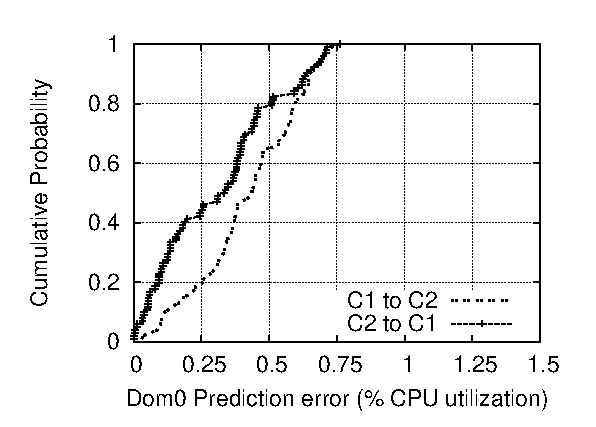
\includegraphics[scale=0.8]{jss-figures/aff-3tier/fwd_3tier_dom0_cdf.eps}
	\caption{Error CDF of Dom0 CPU estimation for C1 to C2 transitions}
	\label{fig:combined}
\end{figure}

\underline{Prediction for two configurations:} The RUBiS\index{RUBiS} 
application run is then performed in
two configurations\textemdash{}(i) \textit{C1}: with proxy server (VM1)
and web-server (VM2) colocated
on PM1 while database server (VM3) hosted alone on PM2, and
(ii) \textit{C2}: with VM1
hosted alone on PM1 while VM2 and VM3 are colocated on PM2.
Resource usage monitoring is performed on both PMs, as before.
Fig.\ref{fig:combined} shows the CDF of prediction error
considering error in prediction for all three PMs, during transition
from \textit{C1} to \textit{C2} and vice-versa.
Maximum error is within 1\% absolute CPU usage for both transitions.

\begin{figure}
	\centering
	\subfloat[\textit{C0}]{\includegraphics[scale=0.475]{jss-figures/rubis-3tier-alone.eps}} ~~~~~~~~~
	\subfloat[\textit{C1}]{\includegraphics[scale=0.475]{jss-figures/rubis-3tier-diff.eps}} \\
	\subfloat[\textit{C2}]{\includegraphics[scale=0.475]{jss-figures/rubis-3tier-same.eps}} ~~~~~~~~~
	\subfloat[\textit{C3}]{\includegraphics[scale=0.475]{jss-figures/rubis-3tier-alone.eps}}
	\caption{Different placements due to series of VM migration steps.}
	\label{fig:migration-steps}
\end{figure}



\underline{Prediction over series of migration steps:}
The above experiment demonstrated that \textit{colocation} and
\textit{dispersion} models can be used as building blocks to do multi-phase
CPU usage prediction for combined transitions. To extend this
further, we consider a series of VM migration steps for this three-tier
application such that each VM migration step results in a different
VM placement and we apply \emph{colocation}\index{Colocation model} and
\emph{dispersion}\index{Dispersion model} prediction models
appropriately to derive CPU usage prediction for each step. The series
of VM migration steps being considered are (Fig.\ref{fig:migration-steps}
shows configurations): (a) \textit{C0}: all 3 VMs on different PMs each
(b) \textit{C1}: VM2 migrates into PM1 and is colocated with VM1
(c) \textit{C2}: VM2 migrates into PM3 and is colocated with VM2
(d) \textit{C3}: VM2 migrates into PM2, same as initial configuration.
For each of the above configurations, we measure CPU utilization
incurred for a RUBiS run with 1000 clients. To test our models, we perform
prediction of CPU usage for the three Dom0 instances (corresponding to
PM1, PM2 and PM3) upon transition from one configuration to the next (e.g.,
\textit{C0}$\rightarrow$\textit{C1},
\textit{C1}$\rightarrow$\textit{C2} and
\textit{C2}$\rightarrow$\textit{C3}).
Maximum error in prediction for each step is listed in
Table \ref{tab:vm-steps-error}.

\begin{table}[h]
	\centering
	\caption{Error in Dom0 prediction over series of VM migrations.}
	% \noindent\makebox[\textwidth]{%
	\begin{tabular}{ |c|c|c|c|} \hline
		\textbf{Transition} & \multicolumn{3}{|c|}{\textbf{Maximum error}} \\
		 & \multicolumn{3}{|c|}{\textbf{in Dom0 prediction}} \\
		 & \multicolumn{3}{|c|}{\textbf{(\% absolute CPU)}} \\ \cline{2-4}
		 & \textbf{PM1} & \textbf{PM2}  & \textbf{PM3} \\ \hline  %\cline{2-9}
		\textit{C0}$\rightarrow$\textit{C1} & 0.75 & NA & NA \\
		\textit{C1}$\rightarrow$\textit{C2} & 1.99 & NA & 0.85 \\
		\textit{C2}$\rightarrow$\textit{C3} & NA & 0.51 & 0.43  \\ \hline
	\end{tabular}
	% }
	\label{tab:vm-steps-error}
\end{table}



Table \ref{tab:vm-steps-error} shows that for every transition step,
Dom0 CPU prediction models perform good prediction and maximum
error is within 2\% absolute CPU utilization. The entry NA in any
particular column implies that prediction is not performed for that
PM during that step. This could be due to one of two reasons: (i) Due to
the VM migration step, the PM has become idle, or (ii) During the
VM migration step, the PM is not the source or destination of
migration.
Thus, we have demonstrated that simple CPU usage prediction models built
on the scale of two VMs can be extended to apply to multi-VM
scenarios as well.


%Though our empirical study is based on Xen virtual machine 
%monitor (VMM\index{VMM}), the approach
%is general enough to be applicable to other virtualization technologies as
%well. For example, in case of KVM\index{KVM} where there is no concept 
%of a privileged
%domain, we expect that the affinity related benefits will be more
%prominently visible in the VM's CPU usage itself, and the above-mentioned modeling will
%prove valuable for CPU usage prediction on colocation/dispersal. We set this
%aside for future work.




